\documentclass[12pt]{article}
% Useful packages that enable things like math symbols and a fancy header

\usepackage{tikz}
\usetikzlibrary{arrows,shapes.gates.logic.US,shapes.gates.logic.IEC,shapes,calc,positioning}
\usepackage{amssymb,amsfonts,amsmath,amsthm}
\usepackage{latexsym}
\usepackage{mathrsfs}
\usepackage{fancyhdr}
\usepackage{outlines}
\usepackage{enumitem}
\usepackage{float}
\usepackage{calc}
\usepackage{graphicx}
\usepackage{svg}

\tikzset{
    between/.style args={#1 and #2}{
         at = ($(#1)!0.5!(#2)$)
    }
}

\tikzset{
    between base/.style args={#1 and #2}{
        between=#1.base and #2.base
    }
}


% Uses the package declared above and makes the page have headers and footers
\pagestyle{fancy}

% Puts a title at the top left
\lhead{CIS 314}
% Puts a title at the center
\chead{Assignment 7}

% Puts a title at the top right
\rhead{Mel McCalla}

% Put's "today's date" in the lower left with the command \today
\lfoot{\today}
\cfoot{\thepage}

%%%%  Some user defined commands that make life easier.  
\newcommand{\be}{\begin{equation}}
\newcommand{\ee}{\end{equation}}
\newcommand{\bea}{\begin{eqnarray}}
\newcommand{\eea}{\end{eqnarray}}
\newcommand{\beas}{\begin{eqnarray*}}
\newcommand{\eeas}{\end{eqnarray*}}
\newcommand{\pa}{\partial}
\newcommand{\la}{\lambda}
\newcommand{\sgn}{\mathrm{sgn}}
\newcommand{\ve}{\varepsilon}
\newcommand{\ra}{\rightarrow}

\renewcommand\qedsymbol{$\blacksquare$}
\DeclareMathOperator{\Ker}{Ker}
\DeclareMathOperator{\M}{M}
\DeclareMathOperator{\PC}{PC}
\DeclareMathOperator{\R}{r}
\DeclareMathOperator{\rA}{rA}
\DeclareMathOperator{\rB}{rB}
\DeclareMathOperator{\valA}{valA}
\DeclareMathOperator{\valB}{valB}
\DeclareMathOperator{\valC}{valC}
\DeclareMathOperator{\valE}{valE}
\DeclareMathOperator{\valP}{valP}


\newlength{\remainingwidth}
\setlength{\remainingwidth}{\textwidth-3cm-24pt}

\begin{document}
\begin{enumerate}
	\item \begin{figure}[htb]
		\centering
		\caption{A diagram of how the instructions are decoded, with their data dependencies.  }
	\tikzstyle{branch}=[fill,shape=circle,minimum size=3pt,inner sep=0pt]
	\begin{tikzpicture}[x=1.5cm,y=1.5cm]
		\node (rcx)	[draw, rectangle]	{\%rcx};
		\node (rbx)	[draw, rectangle, right=of rcx]	{\%rbx};
		\node (rdx)	[draw, rectangle, right=of rbx]	{\%rdx};
		\node (rax)	[draw, rectangle, right=of rdx]	{\%rax};
		\node (xmm1) [draw, rectangle, right=of rax]	{\%xmm1};
		\node (load1) at ($(rbx)+(0,-1)$) [draw, rectangle, rounded corners]		{load};
		\node (load2) at ($(rax)+(0,-1)$) [draw, rectangle, rounded corners]		{load};
		\node (mul)	at ($(load2)+(0,-1)$)		[draw, rectangle, rounded corners]			{mul};
		\node (add1) at ($(rdx)+(0,-2)$)	[draw, rectangle, rounded corners]			{add};
		\node (add2) at ($(xmm1)+(0,-3)$)	[draw, rectangle, rounded corners]			{add};
		\node (cmp)	at ($(rcx)+(0,-3)$)		[draw, rectangle, rounded corners]			{cmp};
		\node (jl)	at ($(cmp)+(0,-1)$)		[draw, rectangle, rounded corners]			{jl};
		\node (rdx_out)	at ($(add1)+(0,-3)$)	[draw, rectangle]		{\%rdx};
		\node (xmm1_out)	at ($(add2)+(0,-2)$)	[draw, rectangle]		{\%xmm1};
		
		\draw (rdx.south)  -- ([yshift=-0.5cm]rdx.south) ;
		\draw[->]
			([xshift=-0.1cm]rbx.south) edge ([xshift=-0.1cm]load1.north)
			([yshift=-0.5cm]rdx.south) node[branch] {}	-- ([xshift=0.1cm, yshift=-0.5cm]rbx.south) edge ([xshift=0.1cm]load1.north)
			([xshift=0.1cm]rax.south) edge ([xshift=0.1cm]load2.north)
			([yshift=-0.5cm]rdx.south) -- ([xshift=-0.1cm, yshift=-0.5cm]rax.south) edge ([xshift=-0.1cm]load2.north)
			([xshift=0.1cm]load2.south) edge ([xshift=0.1cm]mul.north)
			(load1.south) -- ([yshift=-0.5cm] load1.south) -- ([xshift=-0.1cm, yshift=-0.5cm] load2.south) edge ([xshift=-0.1cm]mul.north)
			(rdx) edge (add1)
			(add1) edge (rdx_out)
			(xmm1) edge (add2)
			(mul)	-- ($(mul)+(0,-1)$) edge (add2)
			(add2) edge (xmm1_out)
			(rcx) edge (cmp)
			([yshift=-1.2cm]add1.south) node[branch] {} edge (cmp.east)
			(cmp) edge (jl);	
	\end{tikzpicture}
	\end{figure}
	\item The \texttt{mul} operation and both of the \texttt{add} operations cannot be pipelined, 
	as they have data dependencies on other instructions that have latencies.  The latency for the first floating point add is 3CPE.
	The latency for the integer addition is 1.0CPE.  The latency for the multiplication is 4CPE, 
	as it is a single precision floating point multiplication. 
	So, the lower latency bound for the procedure is 8 CPE.
	\setcounter{enumi}{3}
	\item The unrolled version of the function, \texttt{inner2()}, is faster than \texttt{inner()} in all cases 
	except for very short vectors, especially vectors of length 1.  
	\begin{figure}[htb]
		\centering
		\caption{A graph of the execution time of inner() and inner2()}
 		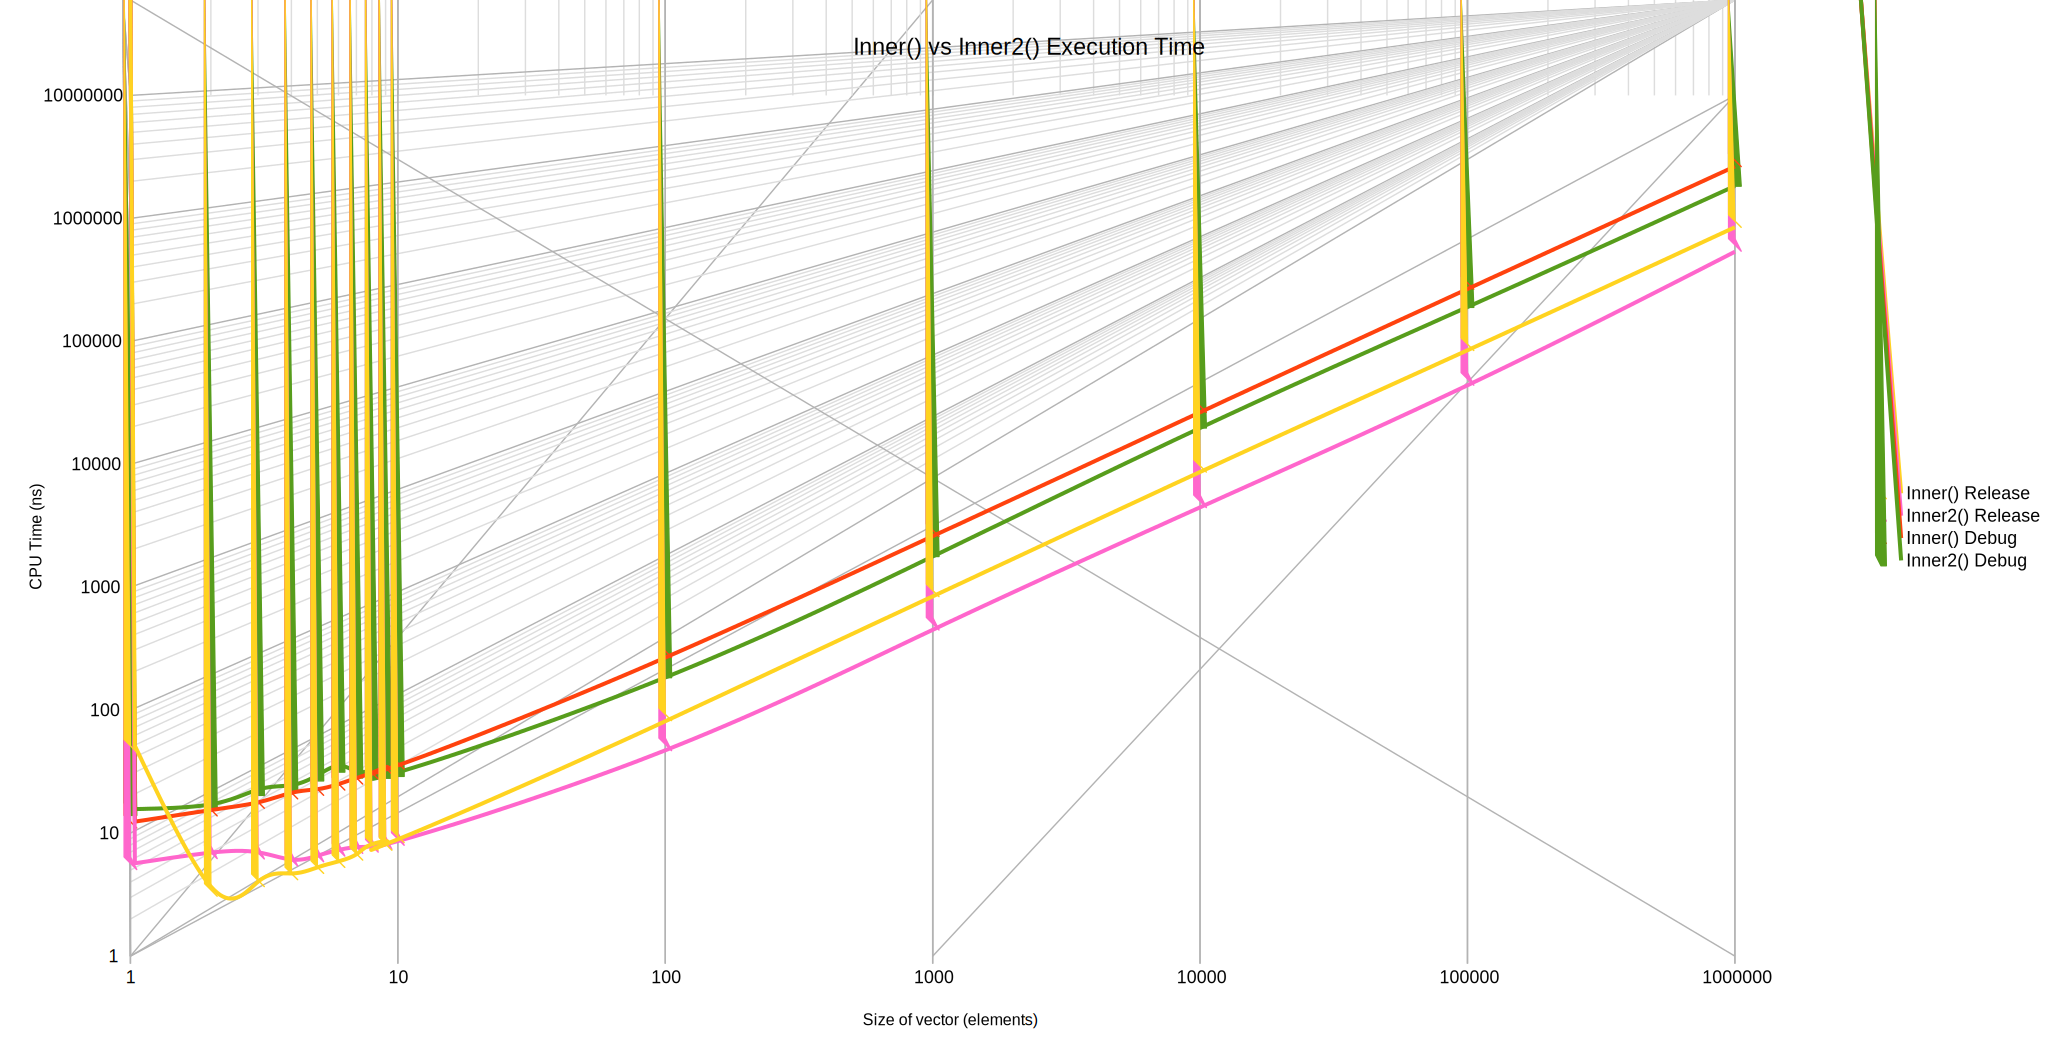
\includegraphics[width=1.0\textwidth]{graph.png}
	\end{figure}
\end{enumerate}

\end{document}